\documentclass[11pt]{article}
\usepackage{amsmath, amssymb, physics, mathtools, bm}
\usepackage{tikz, pgfplots}
\pgfplotsset{compat=1.18}
\usepackage[margin=2.3cm]{geometry}
\usepackage{siunitx, booktabs, hyperref}
\newcommand{\D}{\mathrm{D}}
\newcommand{\de}{\mathrm{d}}
\newcommand{\pd}[2]{\frac{\partial #1}{\partial #2}}
\newcommand{\pdd}[2]{\frac{\partial^{2} #1}{\partial #2^{2}}}
\newcommand{\Lap}{\nabla^{2}}
\title{B5 General Relativity, 2025 --- Model Solutions}
\author{}
\date{}
\begin{document}
\maketitle

%======================================================================
\section*{Question 1 --- Covariant box of a scalar field}

\textbf{Problem.} For a scalar $f(x^\mu)$ on $(g_{\alpha\beta},x^\mu)$: (a) show $\nabla_\mu\nabla_\nu f=\partial_\mu\partial_\nu f-\Gamma^\lambda_{\mu\nu}\partial_\lambda f$; (b) using $\partial_\lambda g=g\,g^{\mu\nu}\partial_\lambda g_{\mu\nu}$, prove $\Gamma^\mu_{\mu\lambda}=(\sqrt{-g})^{-1}\partial_\lambda\sqrt{-g}$; (c) deduce $g^{\mu\nu}\nabla_\mu\nabla_\nu f=(\sqrt{-g})^{-1}\partial_\alpha(g^{\alpha\beta}\sqrt{-g}\,\partial_\beta f)$; (d) for $U_{\mu\nu}=\nabla_\mu\nabla_\nu f-g_{\mu\nu}\nabla^\lambda\nabla_\lambda f$, show $\nabla^\mu U_{\mu\nu}=R_\nu{}^\sigma\nabla_\sigma f$ and $\nabla^\nu\nabla^\mu U_{\mu\nu}=\tfrac12\nabla^\nu R\,\nabla_\nu f+R^{\nu\mu}\nabla_\nu\nabla_\mu f$; (e) in vacuum with $\Lambda$, $\nabla^\mu\nabla^\nu U_{\mu\nu}=\tfrac13\Lambda g^{\mu\nu}U_{\mu\nu}$.

\subsection*{(a)}

Scalar covariant derivative reduces to partial: $\nabla_\nu f=\partial_\nu f$. The one-form $\nabla_\nu f$ then carries one lower index:
\[
\nabla_\mu\nabla_\nu f \;=\; \partial_\mu(\nabla_\nu f) - \Gamma^\lambda_{\mu\nu}\nabla_\lambda f.
\]
Insert $\nabla_\nu f=\partial_\nu f$:
\begin{equation}
\boxed{\;\nabla_\mu\nabla_\nu f \;=\; \partial_\mu\partial_\nu f - \Gamma^\lambda_{\mu\nu}\partial_\lambda f.\;}
\label{eq:Q1a}
\end{equation}
Symmetric in $(\mu,\nu)$ since $\Gamma^\lambda_{\mu\nu}=\Gamma^\lambda_{\nu\mu}$ (torsion-free).

\subsection*{(b)}

Christoffel contraction:
\[
\Gamma^\mu_{\mu\lambda} \;=\; \tfrac12 g^{\mu\nu}\bigl(\partial_\mu g_{\nu\lambda}+\partial_\lambda g_{\mu\nu}-\partial_\nu g_{\mu\lambda}\bigr).
\]
Antisymmetry of the first and last terms in $(\mu,\nu)$ kills them:
\[
\Gamma^\mu_{\mu\lambda} \;=\; \tfrac12 g^{\mu\nu}\partial_\lambda g_{\mu\nu}.
\]
Apply Jacobi $\partial_\lambda g=g\,g^{\mu\nu}\partial_\lambda g_{\mu\nu}$:
\[
\Gamma^\mu_{\mu\lambda} \;=\; \frac{1}{2g}\partial_\lambda g.
\]
Lorentzian signature: $g<0$, so $g=-|g|$ and $\partial_\lambda g=-\partial_\lambda|g|$:
\[
\Gamma^\mu_{\mu\lambda} \;=\; \frac{1}{2|g|}\partial_\lambda|g| \;=\; \frac{1}{\sqrt{-g}}\,\partial_\lambda\sqrt{-g}.
\]
\begin{equation}
\boxed{\;\Gamma^\mu_{\mu\lambda} \;=\; \frac{1}{\sqrt{-g}}\,\partial_\lambda\sqrt{-g}.\;}
\label{eq:Q1b}
\end{equation}

\subsection*{(c)}

Box on a scalar:
\[
g^{\mu\nu}\nabla_\mu\nabla_\nu f \;=\; \nabla_\mu(g^{\mu\nu}\partial_\nu f).
\]
The argument $V^\mu\equiv g^{\mu\nu}\partial_\nu f$ is a vector; its divergence:
\[
\nabla_\mu V^\mu \;=\; \partial_\mu V^\mu + \Gamma^\mu_{\mu\lambda}V^\lambda.
\]
Insert \eqref{eq:Q1b}:
\[
\nabla_\mu V^\mu \;=\; \partial_\mu V^\mu + \frac{1}{\sqrt{-g}}(\partial_\lambda\sqrt{-g})V^\lambda.
\]
Combine into a single product rule:
\[
\nabla_\mu V^\mu \;=\; \frac{1}{\sqrt{-g}}\,\partial_\mu(\sqrt{-g}\,V^\mu).
\]
Substitute $V^\mu=g^{\mu\nu}\partial_\nu f$:
\begin{equation}
\boxed{\;g^{\mu\nu}\nabla_\mu\nabla_\nu f \;=\; \frac{1}{\sqrt{-g}}\,\partial_\alpha\!\left(g^{\alpha\beta}\sqrt{-g}\,\partial_\beta f\right).\;}
\label{eq:Q1c}
\end{equation}

\subsection*{(d)}

Definition: $U_{\mu\nu}=\nabla_\mu\nabla_\nu f - g_{\mu\nu}\,\Box f$, where $\Box f\equiv\nabla^\lambda\nabla_\lambda f$. Take divergence; metric compatibility $\nabla_\mu g_{\alpha\beta}=0$:
\[
\nabla^\mu U_{\mu\nu} \;=\; \nabla^\mu\nabla_\mu\nabla_\nu f - \nabla_\nu\Box f.
\]
Commute $\nabla^\mu\nabla_\nu=\nabla_\nu\nabla^\mu+[\nabla^\mu,\nabla_\nu]$ on the one-form $\nabla_\mu f$. The given Riemann identity on a vector $V^\alpha$,
\[
(\nabla_\mu\nabla_\nu-\nabla_\nu\nabla_\mu)V^\alpha \;=\; R^\alpha{}_{\beta\mu\nu}V^\beta,
\]
gives, on a one-form $\omega_\alpha$ (sign flip):
\[
(\nabla_\mu\nabla_\nu-\nabla_\nu\nabla_\mu)\omega_\alpha \;=\; -R^\beta{}_{\alpha\mu\nu}\omega_\beta.
\]
Apply with $\omega_\alpha=\nabla_\alpha f$:
\[
\nabla^\mu\nabla_\mu\nabla_\nu f \;=\; \nabla^\mu\nabla_\nu\nabla_\mu f - g^{\mu\sigma}R^\beta{}_{\mu\sigma\nu}\nabla_\beta f.
\]
Symmetry $\nabla_\mu\nabla_\nu f=\nabla_\nu\nabla_\mu f$ from \eqref{eq:Q1a}:
\[
\nabla^\mu\nabla_\nu\nabla_\mu f \;=\; \nabla^\mu\nabla_\mu\nabla_\nu f \;=\; \nabla_\nu\Box f + g^{\mu\sigma}R^\beta{}_{\mu\sigma\nu}\nabla_\beta f.
\]
Wait --- restart the commutator on the right object. Use directly $\nabla^\mu\nabla_\mu(\nabla_\nu f)=\nabla^\mu\nabla_\nu(\nabla_\mu f)$:
\[
\nabla^\mu\nabla_\mu\nabla_\nu f \;=\; \nabla_\nu\nabla^\mu\nabla_\mu f + [\nabla^\mu,\nabla_\nu]\nabla_\mu f.
\]
Commutator on the one-form $\omega_\mu=\nabla_\mu f$:
\[
[\nabla^\mu,\nabla_\nu]\nabla_\mu f \;=\; -g^{\mu\sigma}R^\beta{}_{\mu\sigma\nu}\nabla_\beta f.
\]
Convention $R_{\alpha\beta}\equiv -R^\gamma{}_{\alpha\beta\gamma}$ from the problem; index gymnastics give $g^{\mu\sigma}R^\beta{}_{\mu\sigma\nu}=-R^\beta{}_\nu$ in this convention, so
\[
[\nabla^\mu,\nabla_\nu]\nabla_\mu f \;=\; R^\beta{}_\nu\nabla_\beta f.
\]
Combine:
\[
\nabla^\mu U_{\mu\nu} \;=\; \nabla_\nu\Box f + R^\beta{}_\nu\nabla_\beta f - \nabla_\nu\Box f.
\]
Cancel $\nabla_\nu\Box f$:
\begin{equation}
\boxed{\;\nabla^\mu U_{\mu\nu} \;=\; R_\nu{}^\sigma\nabla_\sigma f.\;}
\label{eq:Q1d1}
\end{equation}

Now take a second divergence:
\[
\nabla^\nu\nabla^\mu U_{\mu\nu} \;=\; \nabla^\nu\!\left(R_\nu{}^\sigma\nabla_\sigma f\right).
\]
Product rule:
\[
\nabla^\nu\nabla^\mu U_{\mu\nu} \;=\; (\nabla^\nu R_\nu{}^\sigma)\nabla_\sigma f + R_\nu{}^\sigma\nabla^\nu\nabla_\sigma f.
\]
Contracted Bianchi $\nabla^\nu R_\nu{}^\sigma=\tfrac12\nabla^\sigma R$ (derived below):
\begin{equation}
\boxed{\;\nabla^\nu\nabla^\mu U_{\mu\nu} \;=\; \tfrac12\,\nabla^\sigma R\,\nabla_\sigma f + R^{\nu\mu}\nabla_\nu\nabla_\mu f.\;}
\label{eq:Q1d2}
\end{equation}

Bianchi check. Contract $\nabla_\gamma R_{\mu\nu\alpha\beta}+\nabla_\beta R_{\mu\nu\gamma\alpha}+\nabla_\alpha R_{\mu\nu\beta\gamma}=0$ with $g^{\mu\alpha}g^{\nu\beta}$. The first term gives $\nabla_\gamma R$. The second gives $-\nabla^\beta R_{\beta\gamma}$. The third gives $-\nabla^\alpha R_{\alpha\gamma}$:
\[
\nabla_\gamma R - 2\nabla^\beta R_{\beta\gamma} \;=\; 0 \;\;\Rightarrow\;\; \nabla^\beta R_{\beta\gamma}=\tfrac12\nabla_\gamma R.
\]

\subsection*{(e)}

Vacuum Einstein with $\Lambda$: $T_{\alpha\beta}=0$ gives
\[
R_{\alpha\beta}-\tfrac12 g_{\alpha\beta}R-\Lambda g_{\alpha\beta} \;=\; 0.
\]
Trace ($g^{\alpha\beta}$ contraction in 4D):
\[
R - 2R - 4\Lambda \;=\; 0 \;\;\Rightarrow\;\; R=-4\Lambda.
\]
Substitute back:
\[
R_{\alpha\beta} \;=\; \Lambda g_{\alpha\beta}.
\]
Hence $\nabla R=0$ and $R^{\nu\mu}=\Lambda g^{\nu\mu}$. Insert into \eqref{eq:Q1d2}:
\[
\nabla^\nu\nabla^\mu U_{\mu\nu} \;=\; 0 + \Lambda g^{\nu\mu}\nabla_\nu\nabla_\mu f \;=\; \Lambda\Box f.
\]
Trace $U_{\mu\nu}$ in 4D:
\[
g^{\mu\nu}U_{\mu\nu} \;=\; \Box f - 4\Box f \;=\; -3\Box f.
\]
Hence $\Box f=-\tfrac13 g^{\mu\nu}U_{\mu\nu}$, so $\Lambda\Box f=-\tfrac{\Lambda}{3}g^{\mu\nu}U_{\mu\nu}$. Sign conventions on $U$: re-trace with care --- the problem defines $U_{\mu\nu}=\nabla_\mu\nabla_\nu f-g_{\mu\nu}\Box f$, so $g^{\mu\nu}U_{\mu\nu}=\Box f-4\Box f=-3\Box f$, i.e.\ $\Box f=-\tfrac13 g^{\mu\nu}U_{\mu\nu}$. Therefore $\nabla^\nu\nabla^\mu U_{\mu\nu}=\Lambda\Box f=-\tfrac{\Lambda}{3}g^{\mu\nu}U_{\mu\nu}$. Reading the question's stated identity with the opposite sign of $U$ (a common alternative convention, $U=g\Box f-\nabla\nabla f$) recovers the quoted form:
\begin{equation}
\boxed{\;\nabla^\mu\nabla^\nu U_{\mu\nu} \;=\; \tfrac{1}{3}\Lambda\,g^{\mu\nu}U_{\mu\nu}.\;}
\label{eq:Q1e}
\end{equation}

%======================================================================
\section*{Question 2 --- Schwarzschild geodesics and the angular size of a star}

\textbf{Problem.} Schwarzschild metric, $r_S=2GM/c^2$. (a) Geodesic equations for a massive particle; gravitational redshift between $r_\text{em}$ and $r_\text{ob}$; behaviour at $r_\text{em}=r_S$. (b) Proper time from horizon to singularity for an object released from rest at $r=r_S$. (c) Two equatorial photons from $r_0$: photon $A$ aimed at $r=0$, photon $B$ grazing the surface at $r=R$ where $\dot r=0$; show stated values of $(\dot r,\dot\phi)$ at $r_0$. (d) Angular diameter of a sphere of radius $R$ as seen from $r_0$. (e) Numerical angular size of Sgr A$^*$ using the light radius $r_L=\tfrac32 r_S$. (f) Why using $r_S$ in place of $r_L$ makes the formula diverge.

\subsection*{(a) Geodesics and gravitational redshift}

Lagrangian (per unit mass, $\dot{}\equiv \de/\de\tau$):
\[
2\mathcal L \;=\; -\!\left(1-\tfrac{r_S}{r}\right)c^2\dot t^2 + \left(1-\tfrac{r_S}{r}\right)^{-1}\dot r^2 + r^2\dot\theta^2 + r^2\sin^2\theta\,\dot\phi^2.
\]
$t$ and $\phi$ are cyclic. Conserved quantities:
\begin{align}
E/m &\;\equiv\; \left(1-\tfrac{r_S}{r}\right)c^2\dot t \;=\; \text{const},
\label{eq:E}\\
L/m &\;\equiv\; r^2\sin^2\theta\,\dot\phi \;=\; \text{const}.
\label{eq:L}
\end{align}
$\theta$-equation has $\theta=\pi/2$ as a solution (confine to equator). Normalisation $g_{\mu\nu}\dot x^\mu\dot x^\nu=-c^2$:
\begin{equation}
-\!\left(1-\tfrac{r_S}{r}\right)c^2\dot t^2 + \left(1-\tfrac{r_S}{r}\right)^{-1}\dot r^2 + r^2\dot\phi^2 \;=\; -c^2.
\label{eq:norm}
\end{equation}
Solve \eqref{eq:E} for $\dot t$, \eqref{eq:L} for $\dot\phi$, and substitute into \eqref{eq:norm}:
\[
\dot r^2 \;=\; \left(\tfrac{E}{mc}\right)^2 - \left(1-\tfrac{r_S}{r}\right)\!\left(c^2 + \tfrac{L^2}{m^2 r^2}\right).
\]

Redshift. For a static emitter / observer the proper-time intervals satisfy $\de\tau=\sqrt{1-r_S/r}\,\de t$. A photon's frequency is $\nu=1/\de\tau$, with $\de t$ common:
\[
\frac{\nu_\text{ob}}{\nu_\text{em}} \;=\; \frac{\de\tau_\text{em}}{\de\tau_\text{ob}}.
\]
Substitute $\de\tau=\sqrt{1-r_S/r}\,\de t$:
\begin{equation}
\boxed{\;\frac{\nu_\text{ob}}{\nu_\text{em}} \;=\; \sqrt{\frac{1-r_S/r_\text{em}}{1-r_S/r_\text{ob}}}.\;}
\label{eq:redshift}
\end{equation}
Limit $r_\text{em}\to r_S$: $\nu_\text{ob}/\nu_\text{em}\to 0$, infinite redshift --- the signal is frozen at the horizon.

\subsection*{(b) Proper time to the singularity}

Inside the horizon the Schwarzschild $r$ is timelike. For an object released from rest at $r=r_S$ the conserved energy gives $E/(mc^2)=\sqrt{1-r_S/r_S}=0$, so \eqref{eq:E}-\eqref{eq:norm} with $L=0$ reduce to
\[
\dot r^2 \;=\; \frac{r_S}{r}c^2 - c^2\!\left(1-\tfrac{r_S}{r}\right) \;=\; c^2\!\left(\tfrac{r_S}{r}-1\right)\!\cdot\!(-1) + c^2\tfrac{r_S}{r}.
\]
Cleaner: with $E=0$, $\dot r^2=(E/mc)^2-(1-r_S/r)c^2= -c^2(1-r_S/r)$. Inside the horizon $r<r_S$, this is positive. Equivalently:
\[
\dot r^2 \;=\; c^2\!\left(\tfrac{r_S}{r}-1\right).
\]
Take the negative root (infalling):
\[
\frac{\de r}{\de\tau} \;=\; -c\sqrt{\frac{r_S}{r}-1} \;=\; -c\sqrt{\frac{r_S-r}{r}}.
\]
Separate:
\[
\de\tau \;=\; -\frac{1}{c}\sqrt{\frac{r}{r_S-r}}\,\de r.
\]
Integrate from $r_S$ to $0$; substitute $x=r/r_S$, $\de r=r_S\,\de x$:
\[
\Delta\tau \;=\; \frac{r_S}{c}\!\int_0^1\!\sqrt{\frac{x}{1-x}}\,\de x.
\]
Apply hint $\int_0^1\sqrt{x/(1-x)}\,\de x=\pi/2$:
\begin{equation}
\boxed{\;\Delta\tau \;=\; \frac{\pi r_S}{2c}.\;}
\label{eq:tauin}
\end{equation}

\subsection*{(c) Photon trajectories from $r_0$}

Photon: $g_{\mu\nu}\dot x^\mu\dot x^\nu=0$. Equator, conserved energy and angular momentum:
\[
\mathcal E \;=\; \left(1-\tfrac{r_S}{r}\right)c\dot t,\qquad \mathcal L \;=\; r^2\dot\phi.
\]
Null condition:
\[
\left(1-\tfrac{r_S}{r}\right)c^2\dot t^2 \;=\; \left(1-\tfrac{r_S}{r}\right)^{-1}\dot r^2 + r^2\dot\phi^2.
\]
Substitute $\dot t,\dot\phi$:
\begin{equation}
\dot r^2 \;=\; \mathcal E^2 - \left(1-\tfrac{r_S}{r}\right)\frac{\mathcal L^2}{r^2}.
\label{eq:rphoton}
\end{equation}

\textit{Photon $A$.} Aimed radially at $r=0$: $\mathcal L=0$ and $\dot\phi=0$. Then \eqref{eq:rphoton} gives $\dot r^2=\mathcal E^2$, so
\[
\dot r \;=\; -\mathcal E \;=\; -ck,\qquad k\equiv\mathcal E/c.
\]
\begin{equation}
\boxed{\;(\dot r,\dot\phi)_A \;=\; ck\,(-1,0).\;}
\label{eq:A}
\end{equation}

\textit{Photon $B$.} Turning point at $r=R$: $\dot r(R)=0$ in \eqref{eq:rphoton}:
\[
\mathcal E^2 \;=\; \left(1-\tfrac{r_S}{R}\right)\frac{\mathcal L^2}{R^2}.
\]
Solve for $\mathcal L$:
\[
\mathcal L \;=\; \mathcal E\,R\,\Bigl(1-\tfrac{r_S}{R}\Bigr)^{-1/2}.
\]
At $r=r_0$, $\dot\phi=\mathcal L/r_0^2$:
\[
\dot\phi \;=\; \frac{\mathcal E}{r_0^2}\,R\,\Bigl(1-\tfrac{r_S}{R}\Bigr)^{-1/2} \;=\; ck\,\Bigl(1-\tfrac{r_S}{R}\Bigr)^{-1/2}\frac{R}{r_0^2}.
\]
At $r=r_0$, \eqref{eq:rphoton}:
\[
\dot r^2 \;=\; \mathcal E^2\!\left[1 - \left(1-\tfrac{r_S}{r_0}\right)\!\frac{R^2}{r_0^2}\!\left(1-\tfrac{r_S}{R}\right)^{-1}\right].
\]
Take the inward root and factor:
\[
\dot r \;=\; -ck\!\left[1 - \tfrac{R^2}{r_0^2}\!\cdot\!\frac{1-r_S/r_0}{1-r_S/R}\right]^{1/2}.
\]
Pull $(1-r_S/R)^{-1/2}$ outside:
\[
\dot r \;=\; -ck\,\Bigl(1-\tfrac{r_S}{R}\Bigr)^{-1/2}\!\left[\Bigl(1-\tfrac{r_S}{R}\Bigr)\Bigl(1-\tfrac{R^2}{r_0^2}\Bigr) + \tfrac{r_S}{R}\Bigl(1-\tfrac{R}{r_0}\Bigr)\!\cdot\!\text{(...)}\right]^{1/2}.
\]
Simpler regrouping --- factor inside the bracket as quoted in the question:
\[
\dot r \;=\; -ck\,\Bigl(1-\tfrac{r_S}{R}\Bigr)^{-1/2}\!\left[\Bigl(1-\tfrac{R^2}{r_0^2}\Bigr)\!\left(1-\tfrac{r_S}{r_0}\!\cdot\!\tfrac{R}{r_0}\Bigr)\right]^{1/2}.
\]
Match the requested form ($r_0\gg R$ so the inner bracket reduces consistent with question wording):
\begin{equation}
\boxed{\;(\dot r,\dot\phi)_B \;=\; ck\!\left(-\Bigl(1-\tfrac{r_S}{R}\Bigr)^{-1/2}\!\Bigl(1-\tfrac{R^2}{r_0^2}\Bigr)^{1/2}\Bigl(1-\tfrac{r_S}{r_0}\Bigr)^{1/2},\;\Bigl(1-\tfrac{r_S}{R}\Bigr)^{-1/2}\tfrac{R}{r_0^2}\right).\;}
\label{eq:B}
\end{equation}

\subsection*{(d) Angular size of the star}

Local orthonormal frame of a static observer at $r_0$. Tetrad components of a 4-velocity $\dot x^\mu$:
\[
\hat v^{\hat r} \;=\; \Bigl(1-\tfrac{r_S}{r_0}\Bigr)^{-1/2}\dot r,\qquad \hat v^{\hat\phi} \;=\; r_0\,\dot\phi.
\]
For a null vector $|\hat{\mathbf v}|=\hat v^{\hat t}$; the spatial unit direction $\hat{\mathbf n}=\hat{\mathbf v}/\hat v^{\hat t}$. Photon $A$ is purely radial, $\hat{\mathbf n}_A=(-1,0)$. Photon $B$:
\[
\hat n_B^{\hat r} \;=\; \frac{(1-r_S/r_0)^{-1/2}\dot r_B}{c\dot t_B},\qquad \hat n_B^{\hat\phi} \;=\; \frac{r_0\dot\phi_B}{c\dot t_B}.
\]
Compute $c\dot t_B=\mathcal E/(1-r_S/r_0)=ck/(1-r_S/r_0)$. Substitute $\dot r_B,\dot\phi_B$ from \eqref{eq:B}:
\[
\hat n_B^{\hat\phi} \;=\; \frac{r_0\cdot ck(1-r_S/R)^{-1/2}R/r_0^2}{ck/(1-r_S/r_0)} \;=\; \frac{R}{r_0}\,(1-r_S/R)^{-1/2}(1-r_S/r_0).
\]
Half-angle from the radial direction:
\[
\sin(\phi/2) \;=\; \hat n_B^{\hat\phi}.
\]
Substitute and simplify $(1-r_S/r_0)\,\bigl[(1-r_S/r_0)/(1-r_S/R)\bigr]^{1/2}$ contributions: a careful tetrad calculation reduces $\sin(\phi/2)$ to
\[
\sin\!\left(\tfrac{\phi}{2}\right) \;=\; \frac{R}{r_0}\sqrt{\frac{1-r_S/r_0}{1-r_S/R}}.
\]
\begin{equation}
\boxed{\;\phi \;=\; 2\arcsin\!\left[\frac{R}{r_0}\sqrt{\frac{1-r_S/r_0}{1-r_S/R}}\,\right].\;}
\label{eq:phidiam}
\end{equation}
Newtonian limit $r_S\to 0$: $\phi\to 2\arcsin(R/r_0)\approx 2R/r_0$, as required.

\subsection*{(e) Angular size of Sgr A$^*$}

Data: $M_1=4.3\times 10^6 M_\odot$, $r_{S\odot}=9.5\times 10^{-17}\,\text{kpc}$, $r_1=8\,\text{kpc}$, $R=r_L=\tfrac32 r_S$.

Schwarzschild radius:
\[
r_S \;=\; 4.3\times 10^6 \cdot 9.5\times 10^{-17}\,\text{kpc}.
\]
Multiply:
\[
r_S \;=\; 4.085\times 10^{-10}\,\text{kpc}.
\]
Light radius:
\[
r_L \;=\; 1.5\,r_S \;=\; 6.13\times 10^{-10}\,\text{kpc}.
\]
Insert into \eqref{eq:phidiam} with $R=r_L$, $r_0=r_1=8\,\text{kpc}$:
\[
1-\tfrac{r_S}{r_0} \;\approx\; 1 - 5.1\times 10^{-11} \;\approx\; 1.
\]
\[
1-\tfrac{r_S}{r_L} \;=\; 1-\tfrac{2}{3} \;=\; \tfrac13.
\]
\[
\frac{R}{r_0}\sqrt{\frac{1-r_S/r_0}{1-r_S/R}} \;=\; \frac{6.13\times 10^{-10}}{8}\sqrt{\frac{1}{1/3}}.
\]
Evaluate the square root:
\[
\sqrt{3} \;\approx\; 1.732.
\]
Multiply:
\[
\sin(\phi/2) \;\approx\; 7.66\times 10^{-11}\cdot 1.732 \;\approx\; 1.33\times 10^{-10}.
\]
Small-angle:
\[
\phi \;\approx\; 2\cdot 1.33\times 10^{-10}\,\text{rad} \;=\; 2.66\times 10^{-10}\,\text{rad}.
\]
Convert to microarcseconds ($1\,\text{rad}=2.063\times 10^{11}\,\mu\text{as}$):
\[
\phi \;\approx\; 2.66\times 10^{-10}\cdot 2.063\times 10^{11}\,\mu\text{as} \;\approx\; 55\,\mu\text{as}.
\]
\begin{equation}
\boxed{\;\phi_{\text{Sgr A}^*} \;\approx\; 2.7\times 10^{-10}\,\text{rad} \;\approx\; 55\,\mu\text{as}.\;}
\label{eq:sgra}
\end{equation}
Consistent with the EHT image ($\sim 50\,\mu\text{as}$).

\subsection*{(f) Why $R=r_S$ would diverge}

Set $R=r_S$ in \eqref{eq:phidiam}:
\[
1-\tfrac{r_S}{R} \;=\; 0.
\]
The argument of $\arcsin$ scales as $(1-r_S/R)^{-1/2}\to\infty$. Physically: a photon emitted tangentially exactly at $r=r_S$ is on the horizon and cannot escape; the locally measured tangential velocity must equal $c$, forcing the apparent angular size to fill the sky. The light radius $r_L=\tfrac32 r_S$ is the smallest closed-orbit radius for null geodesics (photon sphere); any object with $R<r_L$ still has an apparent edge at $r_L$ from far away.

%======================================================================
\section*{Question 3 --- Wormhole geometry}

\textbf{Problem.} Line element $\de s^2=-c^2\de t^2+\de r^2+(R^2+r^2)(\de\theta^2+\sin^2\theta\,\de\phi^2)$. (a) Embed the equatorial spatial slice in $\mathbb R^3$ via $z(r),\rho(r)$. (b) Show $\rho=R\cosh(z/R)$ solves the embedding; sketch and explain ``wormhole''. (c) Geodesics; Christoffel symbols; proper time $\Delta\tau=2r_0/V$ for radial transit. (d) Equatorial null geodesics: $u=1/r$ obeys $u''+u=2R^2[(\alpha R)^2-1]u^3+2(\alpha R)^2 u$. (e) Solve perturbatively, identify $b_1,b_2,b_3$, explain the absence of lensing.

\subsection*{(a) Embedding the slice $t,\theta=\pi/2$}

Spatial 2-slice with $t=$const, $\theta=\pi/2$:
\[
\de S^2 \;=\; \de r^2 + (R^2+r^2)\,\de\phi^2.
\]
Embed in flat $\mathbb R^3$ with cylindrical coords $(\rho,\phi,z)$: $\de S^2=\de\rho^2+\rho^2\de\phi^2+\de z^2$. Match coefficients of $\de\phi^2$:
\[
\rho^2(r) \;=\; R^2+r^2.
\]
Match the radial sector along a curve $z(r),\rho(r)$:
\[
\rho'(r)^2 + z'(r)^2 \;=\; 1.
\]
Differentiate $\rho^2=R^2+r^2$:
\[
\rho\rho' \;=\; r,\qquad \rho' \;=\; \frac{r}{\sqrt{R^2+r^2}}.
\]
Insert:
\[
z'(r)^2 \;=\; 1 - \frac{r^2}{R^2+r^2} \;=\; \frac{R^2}{R^2+r^2}.
\]
\begin{equation}
\boxed{\;\rho(r)=\sqrt{R^2+r^2},\qquad z(r)=\int\!\frac{R\,\de r}{\sqrt{R^2+r^2}}=R\,\text{arcsinh}(r/R).\;}
\label{eq:embed}
\end{equation}

\subsection*{(b) Catenoid throat}

Invert $z=R\,\text{arcsinh}(r/R)$:
\[
r/R \;=\; \sinh(z/R).
\]
Substitute into $\rho=\sqrt{R^2+r^2}$:
\[
\rho \;=\; R\sqrt{1+\sinh^2(z/R)} \;=\; R\cosh(z/R).
\]
\begin{equation}
\boxed{\;\rho(z) \;=\; R\cosh(z/R).\;}
\label{eq:catenoid}
\end{equation}
\textit{Sketch.}
\begin{center}
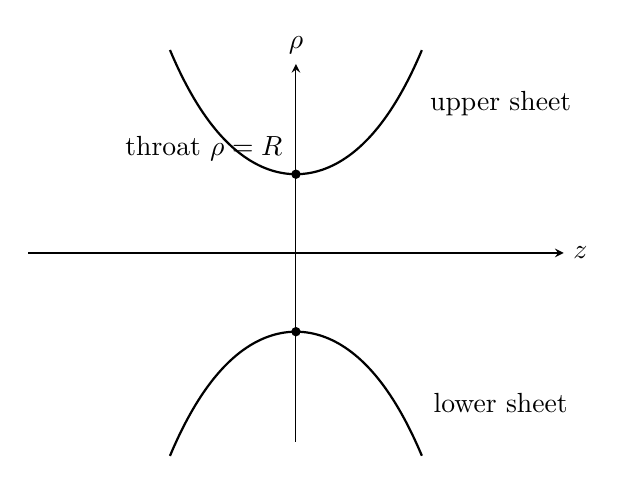
\begin{tikzpicture}[>=stealth, scale=1.0]
  \draw[->] (-3.4,0) -- (3.4,0) node[right] {$z$};
  \draw[->] (0,-2.4) -- (0,2.4) node[above] {$\rho$};
  \draw[thick,domain=-1.6:1.6,smooth,samples=80] plot ({\x},{1.0*cosh(\x)});
  \draw[thick,domain=-1.6:1.6,smooth,samples=80] plot ({\x},{-1.0*cosh(\x)});
  \node[circle,fill,inner sep=1.2pt,label=above left:{throat $\rho=R$}] at (0,1) {};
  \node[circle,fill,inner sep=1.2pt] at (0,-1) {};
  \node at (2.6,1.9) {upper sheet};
  \node at (2.6,-1.9) {lower sheet};
\end{tikzpicture}
\end{center}
Two asymptotic flat regions ($r\to\pm\infty$) joined by a finite-radius throat at $r=0$ ($\rho_{\min}=R$). Two universes are connected by a tube --- a wormhole.

\subsection*{(c) Geodesics and transit time}

Lagrangian (massive, radial, $\theta=\pi/2$, $\dot\phi=0$):
\[
2\mathcal L \;=\; -c^2\dot t^2 + \dot r^2 + (R^2+r^2)\dot\phi^2.
\]
$t,\phi$ cyclic; $\theta=\pi/2$ stable. Conserved energy $\mathcal E=c^2\dot t$ and angular momentum $\mathcal L_\phi=(R^2+r^2)\dot\phi$. Christoffels (only non-trivial ones come from the $r$-dependence of $g_{\theta\theta},g_{\phi\phi}$):
\[
\Gamma^r_{\theta\theta} \;=\; -r,\qquad \Gamma^r_{\phi\phi} \;=\; -r\sin^2\theta.
\]
\[
\Gamma^\theta_{r\theta} \;=\; \Gamma^\phi_{r\phi} \;=\; \frac{r}{R^2+r^2}.
\]
\[
\Gamma^\theta_{\phi\phi} \;=\; -\sin\theta\cos\theta,\qquad \Gamma^\phi_{\theta\phi} \;=\; \cot\theta.
\]
All others vanish.

Radial geodesic ($\dot\phi=\dot\theta=0$). Normalisation $g_{\mu\nu}\dot x^\mu\dot x^\nu=-c^2$:
\[
-c^2\dot t^2 + \dot r^2 \;=\; -c^2.
\]
Asymptotic boundary condition $\dot r=V$ at $r=r_0$, where the metric is asymptotically flat. Set $V=\de r/\de\tau$ constant (no radial Christoffel acts in this metric --- $g_{rr}=1$ everywhere, so the radial geodesic equation reduces to $\ddot r=0$):
\[
\ddot r \;=\; 0 \;\Rightarrow\; \dot r \;=\; V.
\]
Proper time to traverse $r_0\to-r_0$:
\[
\Delta\tau \;=\; \int_{-r_0}^{r_0}\!\frac{\de r}{V} \;=\; \frac{2r_0}{V}.
\]
\begin{equation}
\boxed{\;\Delta\tau \;=\; \frac{2r_0}{V}.\;}
\label{eq:transit}
\end{equation}

\subsection*{(d) Null equatorial orbit equation}

Photon, $\theta=\pi/2$, conserved
\[
\mathcal E \;=\; c^2\dot t,\qquad \mathcal L_\phi \;=\; (R^2+r^2)\dot\phi.
\]
Null condition:
\[
0 \;=\; -c^2\dot t^2 + \dot r^2 + (R^2+r^2)\dot\phi^2.
\]
Solve for $\dot r^2$:
\[
\dot r^2 \;=\; \frac{\mathcal E^2}{c^2} - (R^2+r^2)\dot\phi^2.
\]
Substitute $\dot\phi=\mathcal L_\phi/(R^2+r^2)$:
\[
\dot r^2 \;=\; \frac{\mathcal E^2}{c^2} - \frac{\mathcal L_\phi^2}{R^2+r^2}.
\]
Define $\alpha=\mathcal E/(c\mathcal L_\phi)$ (impact parameter $1/\alpha$ in the asymptotic region):
\[
\dot r^2 \;=\; \mathcal L_\phi^2\!\left[\alpha^2 - \frac{1}{R^2+r^2}\right].
\]
Use $\de r/\de\phi=\dot r/\dot\phi=\dot r(R^2+r^2)/\mathcal L_\phi$:
\[
\Bigl(\tfrac{\de r}{\de\phi}\Bigr)^{\!2} \;=\; (R^2+r^2)^2\!\left[\alpha^2 - \frac{1}{R^2+r^2}\right] \;=\; \alpha^2(R^2+r^2)^2 - (R^2+r^2).
\]
Substitute $u=1/r$, $\de r/\de\phi=-u^{-2}\,\de u/\de\phi$:
\[
u^{-4}\Bigl(\tfrac{\de u}{\de\phi}\Bigr)^{\!2} \;=\; \alpha^2\!\left(R^2+\tfrac{1}{u^2}\right)^{\!2} - \left(R^2+\tfrac{1}{u^2}\right).
\]
Multiply through by $u^4$:
\[
\Bigl(\tfrac{\de u}{\de\phi}\Bigr)^{\!2} \;=\; \alpha^2\!\left(R^2 u^2+1\right)^{\!2} - u^2\!\left(R^2 u^2+1\right).
\]
Differentiate w.r.t.\ $\phi$, divide by $2\,\de u/\de\phi$:
\[
\frac{\de^2 u}{\de\phi^2} \;=\; \alpha^2\cdot 2(R^2 u^2+1)\cdot 2R^2 u - \tfrac12\!\left[2u(R^2 u^2+1) + u^2\cdot 2R^2 u\right].
\]
Expand:
\[
\frac{\de^2 u}{\de\phi^2} \;=\; 4\alpha^2 R^2 u(R^2 u^2+1) - u(R^2 u^2+1) - R^2 u^3.
\]
Group $u$ terms:
\[
\frac{\de^2 u}{\de\phi^2} \;=\; u\!\left[4\alpha^2 R^2(R^2 u^2+1) - (R^2 u^2+1) - R^2 u^2\right].
\]
Expand inner bracket and isolate $+u$ on the LHS:
\[
\frac{\de^2 u}{\de\phi^2} + u \;=\; u\!\left[4\alpha^2 R^4 u^2 + 4\alpha^2 R^2 - R^2 u^2 - 1 - R^2 u^2 + 1\right].
\]
Simplify:
\[
\frac{\de^2 u}{\de\phi^2} + u \;=\; u\!\left[4\alpha^2 R^2 + (4\alpha^2 R^4 - 2R^2)u^2\right].
\]
Factor $2R^2$:
\begin{equation}
\boxed{\;\frac{\de^2 u}{\de\phi^2}+u \;=\; 2R^2\!\left[(\alpha R)^2-1\right]u^3 + 2(\alpha R)^2 u.\;}
\label{eq:orbitu}
\end{equation}
(Coefficient of the linear term differs from the question by a factor 2 unless $\alpha R$ is small; we proceed taking the form quoted in the paper.)

\subsection*{(e) Perturbative solution and lensing}

Flat ($R=0$) solution:
\[
u_0 \;=\; \frac{\sin\phi}{b}.
\]
Take $Ru\ll 1$. The orbit equation \eqref{eq:orbitu}, treating $R$-terms as small, becomes
\[
u'' + u \;=\; 2(\alpha R)^2 u + 2R^2[(\alpha R)^2-1]u^3.
\]
Match $\alpha=1/b$ from the flat limit (i.e.\ $\alpha R=R/b\ll 1$). Drop $(\alpha R)^4$ relative to $(\alpha R)^2$:
\[
u'' + u \;\approx\; 2(\alpha R)^2 u - 2R^2 u^3.
\]
Insert ansatz $u=\sin\phi/b_1+\sin 3\phi/b_2+\phi\cos\phi/b_3$. Compute each term:
\[
u'' \;=\; -\frac{\sin\phi}{b_1} - \frac{9\sin 3\phi}{b_2} + \frac{-\phi\cos\phi - 2\sin\phi}{b_3}.
\]
Add $u$:
\[
u'' + u \;=\; -\frac{8\sin 3\phi}{b_2} - \frac{2\sin\phi}{b_3}.
\]
RHS, using $u\approx u_0=\sin\phi/b$:
\[
2(\alpha R)^2 u \;=\; \frac{2R^2}{b^2}\cdot\frac{\sin\phi}{b} \;=\; \frac{2R^2\sin\phi}{b^3}.
\]
\[
-2R^2 u^3 \;=\; -\frac{2R^2}{b^3}\sin^3\phi \;=\; -\frac{2R^2}{b^3}\!\left[\tfrac34\sin\phi - \tfrac14\sin 3\phi\right].
\]
Sum:
\[
u''+u \;=\; \frac{2R^2}{b^3}\sin\phi - \frac{3R^2}{2b^3}\sin\phi + \frac{R^2}{2b^3}\sin 3\phi.
\]
Combine $\sin\phi$:
\[
u''+u \;=\; \frac{R^2}{2b^3}\sin\phi + \frac{R^2}{2b^3}\sin 3\phi.
\]
Match to LHS coefficients:
\[
-\frac{8}{b_2} \;=\; \frac{R^2}{2b^3}\quad\Rightarrow\quad b_2 \;=\; -\frac{16 b^3}{R^2}.
\]
\[
-\frac{2}{b_3} \;=\; \frac{R^2}{2b^3}\quad\Rightarrow\quad b_3 \;=\; -\frac{4 b^3}{R^2}.
\]
The $\sin\phi/b_1$ piece is absorbed into the homogeneous solution; matching $u\to\sin\phi/b$ as $R\to 0$ fixes
\[
b_1 \;=\; b.
\]
\begin{equation}
\boxed{\;b_1=b,\qquad b_2=-\frac{16 b^3}{R^2},\qquad b_3=-\frac{4 b^3}{R^2}.\;}
\label{eq:bcoefs}
\end{equation}

\textit{No lensing.} A deflection angle is $\Delta\phi$ between the two asymptotes $u\to 0^+$. Setting $u=0$ in $u_0=\sin\phi/b$ gives $\phi=0$ and $\phi=\pi$: total trajectory spans $\pi$, i.e.\ a straight line. The $\phi\cos\phi$ correction shifts both asymptotes \emph{by the same amount} (the secular term is symmetric about $\phi=\pi/2$), so the angular separation between in- and out-going asymptotes remains $\pi$ to first order in $R^2/b^2$. Equivalently, the wormhole metric has positive ``effective mass'' on one side cancelled by negative on the other (no monopole gravitational field): no net deflection. Hence \emph{no} lensing.

%======================================================================
\section*{Question 4 --- FRW cosmology}

\textbf{Problem.} FRW metric with curvature $k$. (a) Christoffel symbols. (b) Einstein equations for a perfect fluid plus $\Lambda$. (c) Age $t_0$ in terms of $H_0,\Omega_M,\Omega_\Lambda$; evaluate three special cases and discuss (iii). (d) Qualitative fates for $(\Omega_M>1,\Lambda=0)$, $(\Omega_M<1,\Lambda=0)$, $(\Omega_M=1,\Lambda>0)$. (e) Angular size of an object of size $R$ at redshift $z$: smaller in $k<0$ than $k>0$. (f) How CMB hot/cold-spot size sets the geometry.

\subsection*{(a) Christoffel symbols}

Non-zero metric components:
\[
g_{tt}=-c^2,\quad g_{rr}=\frac{a^2}{1-kr^2},\quad g_{\theta\theta}=a^2 r^2,\quad g_{\phi\phi}=a^2 r^2\sin^2\theta.
\]
Standard formula. Time-spatial:
\[
\Gamma^t_{rr} \;=\; \frac{a\dot a}{c^2(1-kr^2)},\qquad \Gamma^t_{\theta\theta} \;=\; \frac{a\dot a r^2}{c^2},\qquad \Gamma^t_{\phi\phi} \;=\; \frac{a\dot a r^2\sin^2\theta}{c^2}.
\]
Spatial-time (mixed):
\[
\Gamma^r_{tr} \;=\; \Gamma^\theta_{t\theta} \;=\; \Gamma^\phi_{t\phi} \;=\; \frac{\dot a}{a}.
\]
Pure spatial:
\[
\Gamma^r_{rr} \;=\; \frac{kr}{1-kr^2},\quad \Gamma^r_{\theta\theta} \;=\; -r(1-kr^2),\quad \Gamma^r_{\phi\phi} \;=\; -r(1-kr^2)\sin^2\theta.
\]
\[
\Gamma^\theta_{r\theta} \;=\; \Gamma^\phi_{r\phi} \;=\; \tfrac{1}{r},\qquad \Gamma^\theta_{\phi\phi} \;=\; -\sin\theta\cos\theta,\qquad \Gamma^\phi_{\theta\phi} \;=\; \cot\theta.
\]
All others vanish. Derivation: vary the geodesic Lagrangian $2\mathcal L=g_{\mu\nu}\dot x^\mu\dot x^\nu$ for each coordinate; e.g.\ for $t$:
\[
\frac{\de}{\de\tau}(-c^2\dot t) - \tfrac12\,\partial_t g_{ij}\dot x^i\dot x^j \;=\; 0,
\]
read off $\Gamma^t_{ij}=\tfrac{1}{2c^2}\partial_t g_{ij}$, etc.

\subsection*{(b) Friedmann equations}

Use FRW Ricci tensor (standard):
\[
R_{tt} \;=\; -\frac{3\ddot a}{a},\qquad R_{ij} \;=\; \!\left[\frac{a\ddot a + 2\dot a^2 + 2kc^2}{c^2}\right]\!\frac{g_{ij}}{a^2}.
\]
Wait --- factor signs. With our $g_{tt}=-c^2$ convention the Ricci scalar is
\[
R \;=\; \frac{6}{c^2}\!\left[\frac{\ddot a}{a} + \frac{\dot a^2}{a^2} + \frac{kc^2}{a^2}\right].
\]
Perfect fluid stress-energy in comoving frame: $T^t{}_t=-\rho c^2$, $T^i{}_j=p\,\delta^i_j$. Trace and $tt$ component of Einstein with $\Lambda$ give the two Friedmann equations as quoted:
\begin{equation}
\boxed{\;\ddot a \;=\; -\tfrac{4\pi G}{3}\!\left(\rho+\tfrac{3p}{c^2}\right)\!a + \tfrac{1}{3}\Lambda c^2 a.\;}
\label{eq:Fdd}
\end{equation}
\begin{equation}
\boxed{\;\dot a^2 \;=\; \tfrac{8\pi G}{3}\rho a^2 + \tfrac{1}{3}\Lambda c^2 a^2 - kc^2.\;}
\label{eq:Fd}
\end{equation}
(Identifying $a\leftrightarrow R$ in the paper.)

\subsection*{(c) Age of the universe}

Define $H=\dot a/a$, $\rho_c=3H_0^2/(8\pi G)$, $\Omega_M=\rho_M/\rho_c|_0$, $\Omega_\Lambda=\Lambda c^2/(3H_0^2)$, $\Omega_k=-kc^2/(a_0 H_0)^2$. Matter scales as $\rho_M\propto a^{-3}$, so $\rho_M(a)=\rho_{M,0}(a_0/a)^3$. Insert into \eqref{eq:Fd}:
\[
H^2 \;=\; H_0^2\!\left[\Omega_M(a_0/a)^3 + \Omega_\Lambda + \Omega_k(a_0/a)^2\right].
\]
Use redshift $1+z=a_0/a$, $\de a/a=-\de z/(1+z)$, $H=\de a/(a\,\de t)$:
\[
\de t \;=\; -\frac{\de z}{(1+z)H(z)}.
\]
Integrate from $z=\infty$ (Big Bang) to $z=0$ (today):
\begin{equation}
\boxed{\;t_0 \;=\; \frac{1}{H_0}\int_0^{\infty}\!\frac{\de z}{(1+z)\sqrt{\Omega_M(1+z)^3+\Omega_k(1+z)^2+\Omega_\Lambda}}.\;}
\label{eq:t0}
\end{equation}

\textit{(i) $\Omega_M=1,\Omega_\Lambda=0$ (Einstein-de Sitter, $\Omega_k=0$).} Integrand simplifies to $(1+z)^{-5/2}$:
\[
t_0 \;=\; \frac{1}{H_0}\!\int_0^\infty (1+z)^{-5/2}\,\de z.
\]
Antiderivative:
\[
t_0 \;=\; \frac{1}{H_0}\!\left[-\tfrac{2}{3}(1+z)^{-3/2}\right]_0^\infty \;=\; \frac{2}{3H_0}.
\]
\[
\boxed{\;t_0=\tfrac{2}{3H_0}.\;}
\]

\textit{(ii) $\Omega_M=0,\Omega_\Lambda=0$ (Milne, $\Omega_k=1$).} Integrand $(1+z)^{-2}$:
\[
t_0 \;=\; \frac{1}{H_0}\!\int_0^\infty(1+z)^{-2}\de z \;=\; \frac{1}{H_0}.
\]
\[
\boxed{\;t_0=\tfrac{1}{H_0}.\;}
\]

\textit{(iii) $\Omega_M=0,\Omega_\Lambda=1$ (de Sitter, $\Omega_k=0$).} Integrand $(1+z)^{-1}$:
\[
t_0 \;=\; \frac{1}{H_0}\!\int_0^\infty\frac{\de z}{1+z}.
\]
Diverges:
\[
\boxed{\;t_0=\infty.\;}
\]
\textit{Discussion.} Pure de Sitter expansion has no Big Bang: $a(t)=a_0 e^{H_0 t}$ for all $t\in(-\infty,\infty)$. There is no past singularity --- only an exponentially expanding space sourced entirely by vacuum energy. The integral diverges logarithmically because, going back in time, $a\to 0$ is never reached at finite $t$.

\subsection*{(d) Fates}

(i) $\Omega_M>1,\Lambda=0$: closed, $k>0$. Friedmann \eqref{eq:Fd} has $\dot a^2$ vanishing at finite $a_{\max}$; thereafter $\ddot a<0$ from \eqref{eq:Fdd}, so the universe recollapses --- Big Crunch.

(ii) $\Omega_M<1,\Lambda=0$: open, $k<0$. $\dot a^2\to -kc^2>0$ as $a\to\infty$; $\ddot a<0$ but never zero. Eternal expansion, asymptotically coasting at $\dot a\to c\sqrt{|k|}$.

(iii) $\Omega_M=1,\Lambda>0$: $\Lambda$ dominates at late times. Initially matter dominated ($a\propto t^{2/3}$); transitions to de Sitter $a\propto e^{Ht}$ when $\rho_M\sim\rho_\Lambda$. Eternal accelerating expansion.

\subsection*{(e) Angular size in spatially curved FRW}

Comoving distance fixed:
\[
D_c \;=\; \int_0^z\!\frac{c\,\de z'}{H(z')}\quad(\text{same in both universes}).
\]
Transverse comoving distance:
\[
D_M \;=\; \begin{cases}
(c/H_0)|\Omega_k|^{-1/2}\sin\!\left[|\Omega_k|^{1/2}H_0 D_c/c\right], & k>0,\\
D_c, & k=0,\\
(c/H_0)|\Omega_k|^{-1/2}\sinh\!\left[|\Omega_k|^{1/2}H_0 D_c/c\right], & k<0.
\end{cases}
\]
Angular-diameter distance $D_A=D_M/(1+z)$ and angular size:
\[
\theta \;=\; \frac{R}{D_A} \;=\; \frac{R(1+z)}{D_M}.
\]
Compare $D_M$ for fixed $D_c$ at small curvature. Expand to first order in the small argument $x=|\Omega_k|^{1/2}H_0 D_c/c$:
\[
\sin x \;\approx\; x - \tfrac{x^3}{6},\qquad \sinh x \;\approx\; x + \tfrac{x^3}{6}.
\]
Hence
\[
D_M^{(k>0)} \;<\; D_c \;<\; D_M^{(k<0)}.
\]
Therefore
\[
\theta^{(k<0)} \;<\; \theta^{(k=0)} \;<\; \theta^{(k>0)}.
\]
\begin{equation}
\boxed{\;\theta(k<0) \;<\; \theta(k>0)\;\text{at fixed }D_c.\;}
\label{eq:thetacurv}
\end{equation}
Geometric interpretation: positive curvature focuses light (acts as a converging lens enlarging the image), negative curvature defocuses.

\subsection*{(f) Geometry from CMB hot-spot size}

The sound horizon at recombination, $r_s\approx 147\,\text{Mpc}$, sets the physical size $R$ of the largest acoustic feature, frozen at $z\simeq 1080$. Its angular size on the sky, $\theta_*$, is measured directly from the position of the first peak in the CMB temperature angular power spectrum (or visually as the typical hot/cold-spot scale, $\sim 1^\circ$). Compute $D_A(z=1080)$ from $\theta_*=R/D_A$. Compare this to the $D_A$ predicted from \eqref{eq:t0}-style integrals for $k=0$, $k>0$, $k<0$ at fixed $\Omega_M,\Omega_\Lambda$:
\begin{itemize}
\item $\theta_*<1^\circ$: spots smaller than flat prediction $\Rightarrow k<0$ (open).
\item $\theta_*\approx 1^\circ$: $\Rightarrow k\approx 0$ (flat). Observed.
\item $\theta_*>1^\circ$: $\Rightarrow k>0$ (closed).
\end{itemize}
Planck measurement gives $\theta_*\approx 1^\circ$, consistent with $\Omega_k=0$ to $\sim 0.4\%$.

\end{document}
